\documentclass{article}
\usepackage{graphicx}
\usepackage{listings}
\usepackage{hyperref}
\usepackage{datetime}
\begin{document}

\title{Dynamics of mass, spring and damper system}
\author{Dinesh A(153010009)}
% \today
\maketitle


\section{Introduction}
To study a motion of a mass with given initial state connected to a
wall with a spring and a damper can be done using differential
equations. Lets assume a mass (m) is connected to a wall with spring
of stiffness k and a damper of constant c. Assume that the mass m is
given a initial displacement of x and released with zero velocity
\begin{figure}
  \centering
  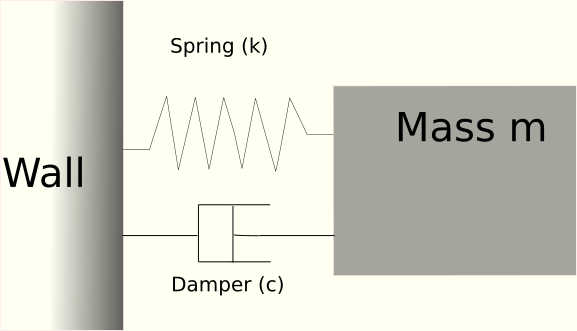
\includegraphics[width=0.7\linewidth]{mass_damper}
  \caption{Mass spring damper system}
\label{fig:msd}
\end{figure}

\subsection{Forces on mass}
Since the mass attached to a spring and a damper, there will be two forces 
on the mass when it is disturbed from its equilibrium position.

\subsubsection{Hooke's law}

Hooke's law  states that if a spring is  elongated with  an amount  x, then
\label{fig:hookes_law}force exerted by the spring on the object elongating is

\begin{equation}
  F_s = -kx
\end{equation}

\begin{figure}
  \centering
  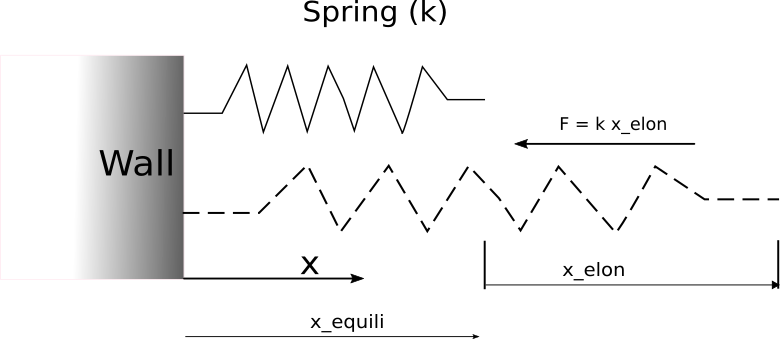
\includegraphics[width=0.7\linewidth]{hookes_law}
  \caption{Force by an elongated spring}
\end{figure}

\subsubsection{Damping force}

The force from the damper to reduce the energy of
the mass is 
\begin{equation}
  F_d = -c\frac{dx}{dt}
\end{equation}

The total force on the mass neglecting gravity at a given time is

\begin{equation}
  F_{total} = F_s + F_d
\end{equation}


\section{Applying Newton's second law}
From Newton's second law the equation of motion\cite{rao} can be written as
\begin{equation}
m \frac{d^{2}x}{dt^{2}} = F_{{total}} 
\end{equation}

This second order differential equation can be decoupled into two first
order differential equations and velocity and position can be
calculated using a scipy integrator for time t. 

\begin{eqnarray}
\frac{dx}{dt} &=& v \\
\frac{d^{2}x}{dt^{2}} = v &=& F_{total}/m 
\end{eqnarray}

\section{Results}

Using the following python code the velocity and position can be
plotted against the time t.

\lstinputlisting{mass_damper.py}

\begin{figure}
  \centering
  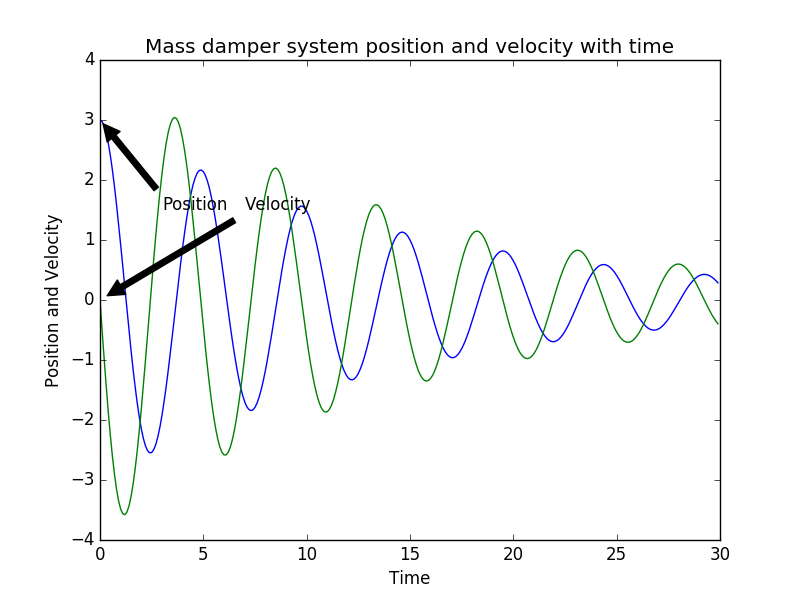
\includegraphics[width=0.9\linewidth]{result}
  \caption{Position and velocity of mass damper spring system with time}
\label{fig:result}
\end{figure}


\nocite{den}
\bibliographystyle{plain}
\bibliography{lit.bib}


\end{document}
%%% Local Variables:
%%% mode: latex
%%% TeX-master: t
%%% End:
